\documentclass[12pt, twocolumn]{article}
\usepackage{lmodern}

\usepackage{graphicx}
\usepackage{adjustbox}
\usepackage{tabularx}
\usepackage{subcaption}
\usepackage{minted}
%\usepackage{authblk}
% \usepackage{markdown}
% \usepackage[]{appendix}
\usepackage{amsmath}
\usepackage[printonlyused, nohyperlinks]{acronym}
\usepackage{amssymb}
\usepackage{listings}
\usepackage{booktabs}
% \input{snippets/tikz.tex}
% \usepackage[authoryear]{natbib}
\usepackage{float}
\usepackage{glossaries}
%\usepackage[hyphens]{url}
%\usepackage[german]{babel}
\usepackage[british]{babel}
\usepackage[utf8]{inputenc} %für Umlaute äüöß
\usepackage{array}
\usepackage[bookmarks]{hyperref}
\graphicspath{{img/}}
\usepackage{lmodern}
%avoid breaking across pages
\interfootnotelinepenalty=10000
\usepackage{xcolor}
\usepackage{multirow}
\usepackage{multicol}
\usepackage{tabu}
\usepackage{colortbl}
\usepackage{lipsum}

\newcommand{\RomanNumeralCaps}[1]
    {\MakeUppercase{\romannumeral #1}}


%adapting the article class to Ketter requirements
%\usepackage{showframe}
%\usepackage{setspace}
%\onehalfspacing
%\lstset{
%    basicstyle=\footnotesize,        % the size of the fonts that are used for the code
%    breakatwhitespace=false,         % sets if automatic breaks should only happen at whitespace
%    breaklines=true,                 % sets automatic line breaking
%    captionpos=b,                    % sets the caption-position to bottom
%    % deletekeywords={...},            % if you want to delete keywords from the given language
%    % escapeinside={\%*}{*)},          % if you want to add LaTeX within your code
%    % frame=single,                    % adds a frame around the code
%    keepspaces=true,                 % keeps spaces in text, useful for keeping indentation of code (possibly needs columns=flexible)
%    %  keywordstyle=\color{blue},       % keyword style
%    numbers=left,                    % where to put the line-numbers; possible values are (none, left, right)
%    numbersep=5pt,                   % how far the line-numbers are from the code
%    rulecolor=\color{black},         % if not set, the frame-color may be changed on line-breaks within not-black text (e.g. comments (green here))
%    showspaces=false,                % show spaces everywhere adding particular underscores; it overrides 'showstringspaces'
%    showstringspaces=false,          % underline spaces within strings only
%    showtabs=false,                  % show tabs within strings adding particular underscores
%    stepnumber=1,                    % the step between two line-numbers. If it's 1, each line will be numbered
%    tabsize=2,                       % sets default tabsize to 2 spaces
%}

%\makeglossaries
%\printglossaries

\newglossaryentry{economiccontrol}
{
	name=Economic Control,
	description={Control by the broker over customers regulatable devices such as storage devices or production devices}
}

\newglossaryentry{balancingcontrol}
{
	name=Balancing Control,
	description={Control which is managed by the \ac{DU} and performs the same as \gls{economiccontrol} activities.}
}




\usepackage{easylist}
\usepackage{hanging}
\usepackage{hyperref}
\usepackage{blindtext}
\usepackage{tipa}
\usepackage[left=2.5cm, top=2cm, bottom=2cm, right=2cm]{geometry}

\begin{document}

\begin{titlepage}

\begin{center}

\Huge{What methods should a trade uniion adopt to achieve its objectives?}
\vspace{10mm}

\normalsize{\today}


\vspace{10mm}


\begin{figure}[!h]
    \centering
    
\includegraphics[width=0.5\textwidth]{logo.png}
\end{figure}

\vspace{5mm}

\small{Industrial Managment\\ ECE -1}
\vspace{5mm}
\small{Department of Electronics and Communication And Engineering\\ Bharati Vidyapeeth College Of Engineering\\ }


\begin{multicols}{2}
\small{Ashish Arora - 01511502818} \\
\small{Ashwin Goyal - 01711502818} \\
\small{Bhavesh Dangwal - 01811502818} \\
\small{Bhupesh Bhatt - 01911502818} \\
\small{Deepanshu Tyagi - 02011502818} \\
\small{Divyanshu Bist - 02211502818} \\
\small{Ekansh Bhatnagar - 02311502818} \\
\small{Eshan Singh - 02411502818} \\
\small{Gagan Gupta - 02511502818} \\
\small{Gautam Manocha - 02611502818} \\
\end{multicols}

\end{center}

\end{titlepage}

\pagenumbering{Roman}

\onecolumn
\setcounter{tocdepth}{3}
\tableofcontents{}
\newpage



\twocolumn[

\begin{@twocolumnfalse}
\pagenumbering{arabic}
\begin{abstract}
	Semiconductors and microprocessors are essential to modern technology;
	their absence would halt every aspect of modern life. Advances and improvements
	in the semiconductor industry have fueled the technological revolution of the
	1990s. The decrease in the cost and size of transistors allowed for an every
	increasing amount of transistors to be put onto a silicon chip, thereby allowing
	for faster processors.
	The ability to fit more transistors on a silicon wafer approximately follows
	Moore’s Law, which is named after Gordon Moore, co-founder of Intel Corporation.
	Moore’s Law states that the number of transistors on a silicon chip doubles every 18-24 months.
\end{abstract}
\end{@twocolumnfalse}
]



\section{Introduction}

Intel Corporation was founded on July 18, 1968 by semiconductor pioneers
Robert Noyce and Gordon Moore (of Moore's law) and is associated with
the executive leadership and vision of Andrew Grove. The company's name
was conceived as portmanteau of the words \emph{int}egrated and
\emph{el}ectronics, with co-founder Noyce having been a key inventor of
the integrated circuit (the microchip). The fact that "intel" is the
term for intelligence information also made the name appropriate. Intel
was an early developer of SRAM and DRAM memory chips, which represented
the majority of its business until 1981. Although Intel created the
world's first commercial microprocessor chip in 1971, it was not until
the success of the personal computer (PC) that this became its primary
business.

Intel supplies microprocessors for computer system manufacturers such as
Apple, Lenovo, HP, and Dell. Intel also manufactures motherboard
chipsets, network interface controllers and integrated circuits, flash
memory, graphics chips, embedded processors and other devices related to
communications and computing.


Intel Corporation is an American multinational corporation

and technology company headquartered in Santa Clara, California, in Silicon
Valley. It is the world's largest and highest-valued semiconductor chip
manufacturer on the basis of revenue, and is the developer of the x86
series of microprocessors, the processors found in most personal
computers (PCs). Intel ranked No. 46 in the 2018 \emph{Fortune} 500 list
of the largest United States corporations by total revenue. Intel is
incorporated in Delaware.

\begin{figure}[ht!]
	\centering

\includegraphics[width=2.72896in,height=1.08604in]{media/image2.jpeg}
\end{figure}



\begin{figure}[ht!]
	\centering
	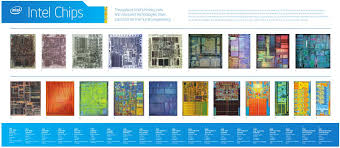
\includegraphics[scale=0.5]{media/timeline.jpg}
	\caption{Timeline of Intel Processors}
\end{figure}


\hypertarget{bit}{%
\section{1971-1981: 4004 (8-bit)}\label{bit}}

The 4004, manufactured from 1971 to 1981, was the first commercially
available processor as well as the first complete CPU on a single chip.
The chip was packaged in a 16-pin ceramic dual in-line package and was
initially released with a clock speed of 108 KHz (and scaled up to 740
KHz). Produced in a 10 μm (10,000 nm) process, the 4004 had 2,300
transistors and delivered a performance of 0.07 MIPS.

The 8-bit 8008 replaced the 4004 in 1972 with 0.5 to 0.8 MHz clock speed
and 3,500 transistors, and was primarily used in the TI 742 computer.
The 8080 followed in 1974 with 4,500 transistors in 6,000 nm with up to
2 MHz and became famous for being used in the Altair 8800 as well as in
Boeing's AGM-86 cruise missile.

None of these chips were sold in considerable volumes.

\begin{figure}[h!]
	\centering
	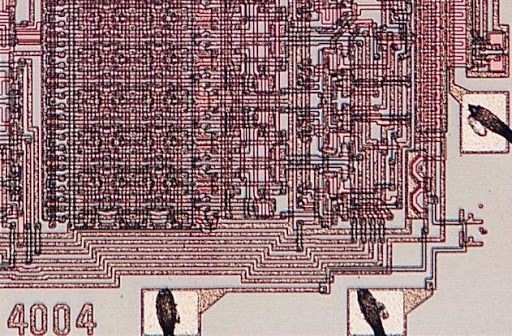
\includegraphics[scale=0.5]{media/image5.jpeg}
\end{figure}


\hypertarget{iapx-86-8086-8088-and-80186-16-bit}{%
\section{1978-1982: iAPX 86 -- 8086, 8088 and 80186
(16-bit)}\label{iapx-86-8086-8088-and-80186-16-bit}}

The 8086, also known as the iAPX 86, was Intel's first commercial 16-bit
CPU and is considered to be the chip that launched the era of x86
processors. With 29,000 transistors built in a 3,000 nm design, the 8086
was clocked from 5 to 10 MHz and achieved up to 0.75 MIPS in computers
such as the IBM PS/2.

The IBM 5150, the first PC, came with the 8088 (5-8MHz), which was
identical to the 8086 with the exception of its 8-bit internal bus. In
1982, Intel launched the 80186 CPU, which was also based on the 8086,
but was built in 2,000 nm and hit more than 1 MIPS at 6 MHz clock speed.
The Tandy 2000 was among the first PCs that used the 80186.


\begin{figure}[h!]
	\centering
	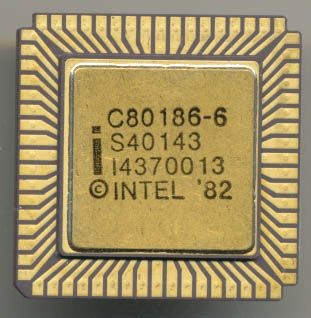
\includegraphics[scale=0.5]{media/image8.jpeg}
\end{figure}

% \hypertarget{iapx-432}{%
% \section{1981: iAPX 432}\label{iapx-432}}

% The iPAX 432 is one of the very few Intel processor designs that flopped
% and Intel does not talk about anymore. Other future ill-fated processor
% designs included the i860/i960 in the early 1990s as well as the highly
% integrated Timna processor in 2000.

% Introduced in 1981, the 432 was Intel's first 32-bit design -- an
% amazingly complex design for its time that integrated hardware-based
% multitasking and memory management features. Designed for high-end
% systems, the downfall of the 4-8 MHz 432 was the fact that it was much
% more expensive to produce and slower than the emerging 80286 design.

% While the 432 was originally designed as a replacement for the 8086
% series, the project was ended in 1982.

% \begin{figure}[h!]
% 	\centering
% 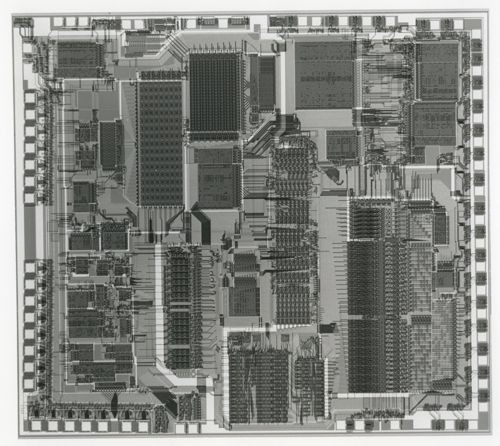
\includegraphics[width=2.0331in,height=1.81187in]{media/image9.jpeg}
% \end{figure}

% \hypertarget{section}{%
% \section{1982: 80286}\label{section}}

% Intel's 80286 debuted with memory management and wide protection
% abilities, and reached clock speeds up to 25 MHz with a performance of
% more than 4 MIPS in 1991. This processor was popular in IBM-PC AT and AT
% PC clones. The chip was manufactured in 1500 nm and included 134,000
% transistors.

% The 80286 is remembered as the Intel processor that provided the highest
% performance gain over its predecessor and one of the most cost-efficient
% processors Intel ever produced. In 2007, Intel stressed that only the
% new Atom processor was about as cost-efficient as the 80286 25 years earlier.

% \begin{figure}[h!]
% 	\centering
% 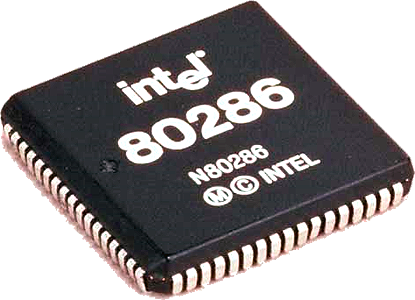
\includegraphics[width=2.41666in,height=1.75in]{media/image10.png}
% \end{figure}

% \hypertarget{and-376}{%
% \section{1985-1994: 386 and 376}\label{and-376}}

% The 32-bit era began with the release of the 386DX CPU in 1985. With
% 275,000 transistors (1,500 nm) and clock speeds ranging from 16 to 33
% MHz, the CPU hit up to 11.4 MIPS.

% In 1988, Intel followed up with the 1,000 nm 386SX, which had a narrower
% 16-bit bus to target mobile and low-cost desktop computing systems.
% Although the 386SX remained fully 32-bit capable internally, the data
% bus was cut down to 16 bits to simplify circuit board layout and reduce
% costs. Additionally, although not critical at the time, only 24 pins
% were connected to the 386SX's address bus, which effectively limited it
% to addressing 16MB of memory.

% Both of the chips lacked a math coprocessor, and due to early problems
% with the i387 coprocessor not being production-ready in time for the
% 80386, both chips had to fall back to the 80287 as their math
% coprocessor until the 80387 was released to the market.

% Intel's first notebook chip, the 386SL, arrived in 1990 as a highly
% integrated design with on-chip cache, bus, and memory controller. The
% processor had 855,000 transistors and ran between 20 and 25 MHz. The 376
% (1989) and 386EX (1994), both for embedded systems, completed the
% 376/386 processor family. Despite it becoming obsolete as a personal
% computer CPU in the early '90s, Intel continued to manufacture the 80386
% family until September of 2007, due to market demand for the chip to be
% used in embedded systems and the chip's wide use by the aerospace
% industry.


% \begin{figure}[ht!]
% 	\centering
% 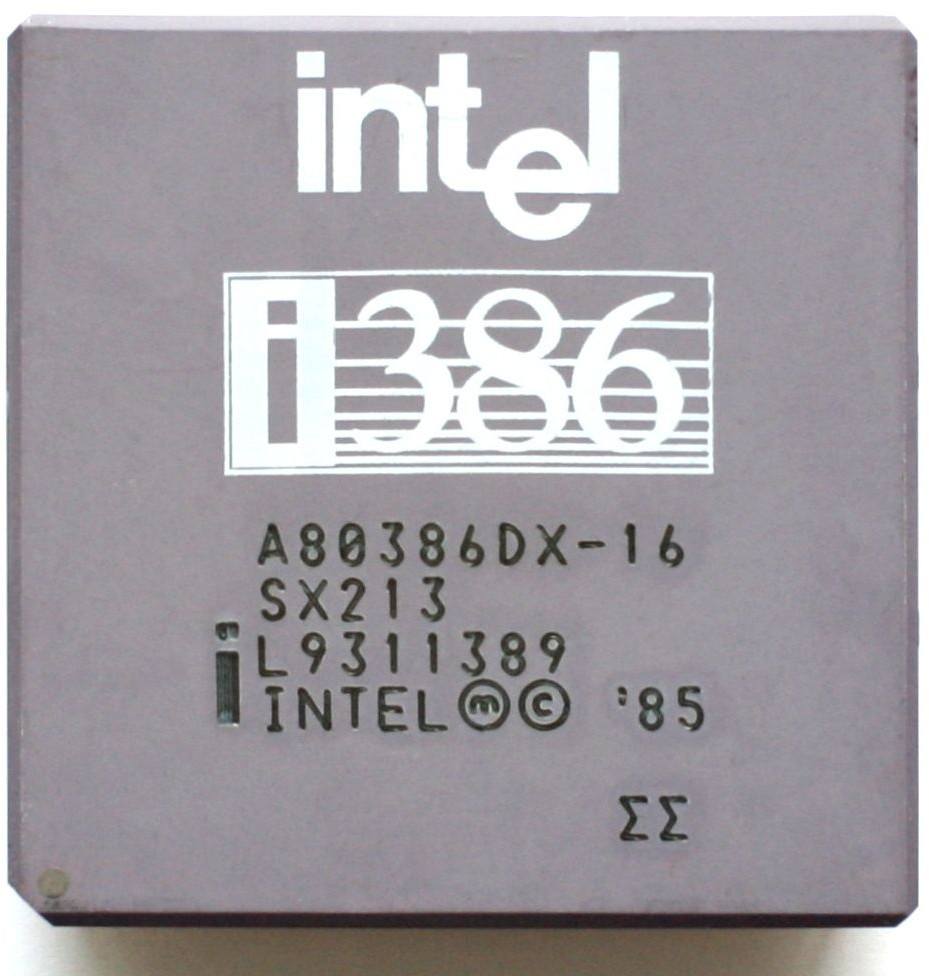
\includegraphics[width=1.84128in,height=1.93167in]{media/image11.jpeg}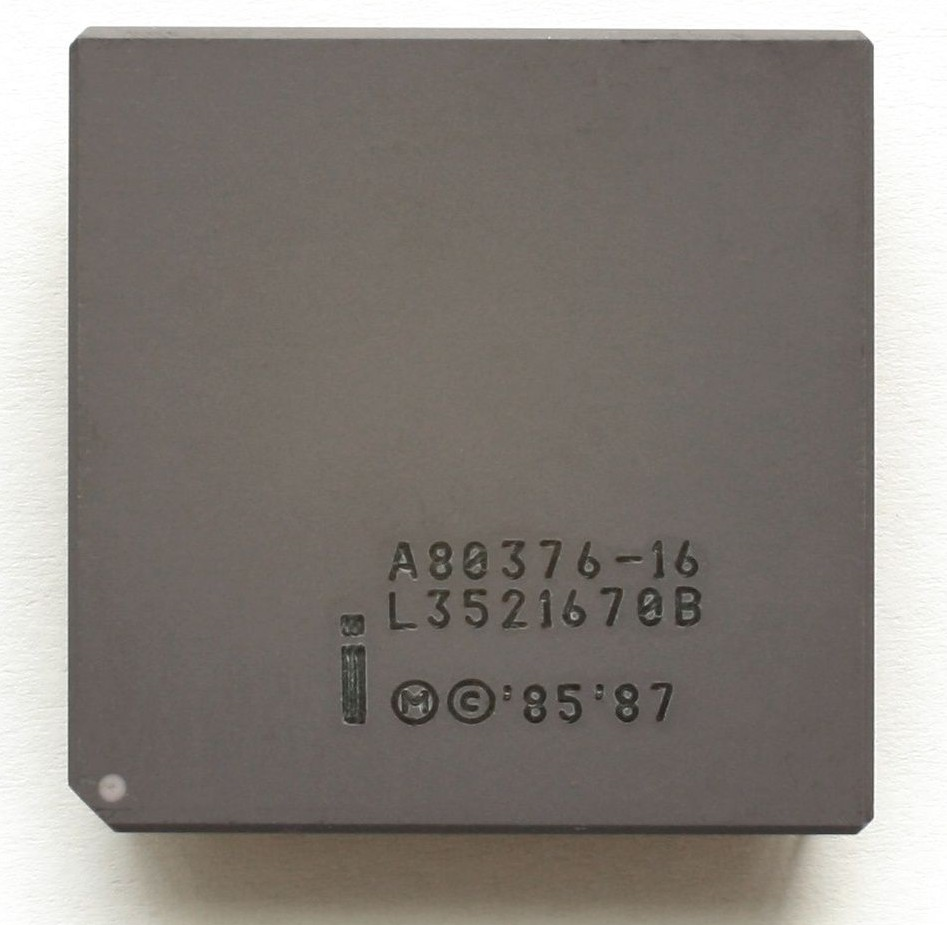
\includegraphics[width=1.96722in,height=1.92708in]{media/image12.jpeg}
% \end{figure}

% \hypertarget{and-i860}{%
% \section{1989: 486 and i860}\label{and-i860}}

% The 486, designed under the guidance of Pat Gelsinger, today's CEO of
% VMware, drove Intel through its greatest phase of growth. The 1,000 nm
% and 800 nm design was launched as 486DX with 25 to 50 MHz, included 1.2
% million transistors and delivered 41 MIPS. The low-end 486SX (a 486DX
% with disabled math co-processor) followed in 1991 with 16 to 33 MHz.

% In 1992, Intel introduced an update as the 486DX2 (SX2) with up to 66
% MHz, while the 486SL as an enhanced 486SX was offered for notebooks (up
% to 33 MHz, 800 nm, 1.4 million transistors). The final stage of the 486
% series was the 486DX4 with up to 100 MHz, which was marketed as an
% economical solution for those who did not want to spend more money on
% the new Pentium systems. The DX4 was built in a 600 nm process, had

% 1.6 million transistors and was rated at 70.7 MIPS.

% 1989 was also the release year of the i860, Intel's attempt to enter the
% RISC processor race and the company's second major shot at the high-end
% computer segment. The i860 and i960 never succeeded and were canceled in
% the early 1990s.

% \begin{figure}[ht!]
% 	\centering
% 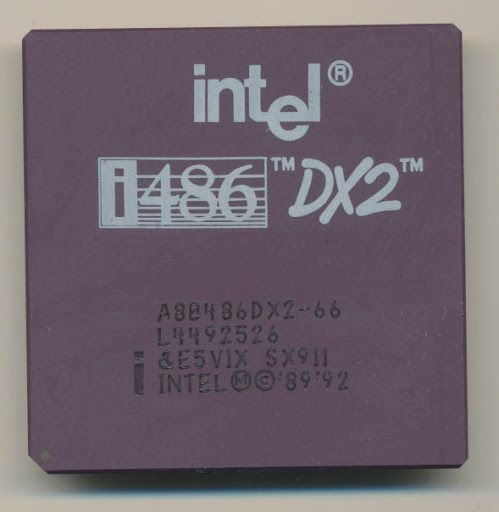
\includegraphics[width=2.44401in,height=2.50667in]{media/image13.jpeg}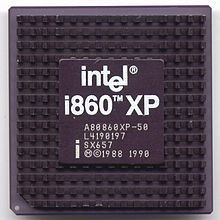
\includegraphics[width=2.49792in,height=2.49792in]{media/image14.jpeg}
% \end{figure}

% \hypertarget{pentium-p5-i586}{%
% \section{1993: Pentium (P5, i586)}\label{pentium-p5-i586}}

% The original Pentium was introduced in 1993. In 2005, there were rumors
% that Intel would drop the name in favor of the new Core brand, but the
% Pentium brand lives on. The brand is an important part of Intel's
% history and departure from the 286/386/486 processor numbers; Intel
% reportedly chose a word to be able to protect the trademark against AMD,
% which also offered 486-labeled processors.

% The P5 Pentium launched with 60 MHz in 1993 and was available with up to
% 200 MHz (P54CS) in 1996. The original 800 nm design had 3.1 million
% transistors, but scaled to 3.3 million in the 350 nm 1996 design. The
% P55C was announced in 1997 with MMX (Multimedia Extensions) and expanded
% the processor design to 4.5 million transistors and 233 MHz clock speed.
% The mobile version of the Pentium MMX remained available until 1999 and
% reached 300 MHz.

% \begin{figure}[ht!]
% 	\centering
% 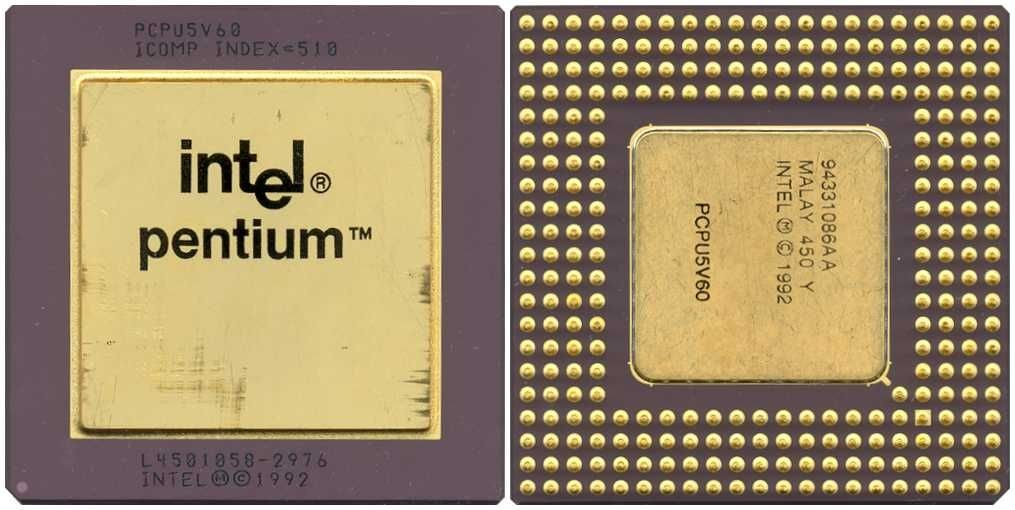
\includegraphics[width=3.05026in,height=1.54062in]{media/image15.jpeg}
% \end{figure}

\hypertarget{pentium-pro-p6-i686}{%
\section{1995: Pentium Pro (P6, i686)}\label{pentium-pro-p6-i686}}

the Pentium Pro was a largely misunderstood processor. Many believed
that the Pro was intended to replace the P5. However, as a precursor to
the Pentium II Xeon, the Pentium Pro was tailored to deal with workloads
typical for servers and workstations.

The Pentium Pro's architecture was different from the regular Pentiums
and supported out of order execution, the Pentium Pro had a 36-bit
address bus, which supported up to 64GB of memory. The Pentium Pro was
built in 350 nm, had 5.5 million transistors, and came in several
variants with clock speeds ranging from 150 and 200 MHz.

\begin{figure}[ht!]
	\centering
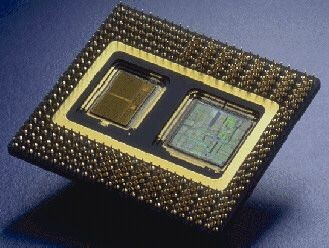
\includegraphics[scale=0.5]{media/image16.jpeg}
\end{figure}

\hypertarget{pentium-ii-and-pentium-ii-xeon}{%
\section{1997: Pentium II and Pentium II
Xeon}\label{pentium-ii-and-pentium-ii-xeon}}

The Pentium II was a consumer-focused processor developed on top of the
sixth-generation P6 architecture, and the first Intel CPU that was
delivered in a

cartridge-like slot module and not a socket device. The Pentium II had 2
million more transistors (7.5 million) than the P6, significantly
improving 16-bit execution, which was a problem in the initial P6
release, and carried on the MMX instruction set that was introduced with
the Pentium.

The Pentium II was released with the 350 nm Klamath core (233 and 266
MHz). Deschutes arrived as a shrink to 250 nm and clock speeds up to 450
nm in 1998, and was also offered as Pentium II Overdrive as an upgrade
option for the Pentium Pro. Mobile Pentium II processors got the 250 nm
Tonga and 250 nm and 250nm/180 nm Dixon cores. In the same year, Intel
also offered the Deschutes core as a Pentium II Xeon with larger cache
and dual-processor support.

\begin{figure}[ht!]
	\centering
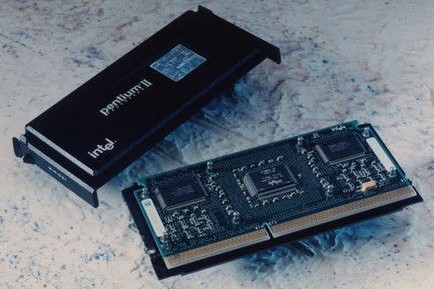
\includegraphics[width=2.62429in,height=1.74604in]{media/image17.jpeg}
\end{figure}

\hypertarget{celeron}{%
\section{1998: Celeron}\label{celeron}}

Celeron was launched in 1998 as a variant of the Pentium II processor.
While Celerons are based on the company's current processor technology,
they usually come with substantial downgrades, such as less cache
memory, which positions them as processors that are just "good enough"
for the most basic PC applicationsThe first Celeron series was based on
the 250 nm Covington core for desktops and the 250 nm Mendocino core for
notebooks. The processors were available from 266 to 300 MHz on the
desktop and up to 500 MHz on the mobile side, and were updated well into
the days of the succeeding Pentium III. Today's Celerons are based on
Sandy Bridge architecture.

\begin{figure}[ht!]
	\centering
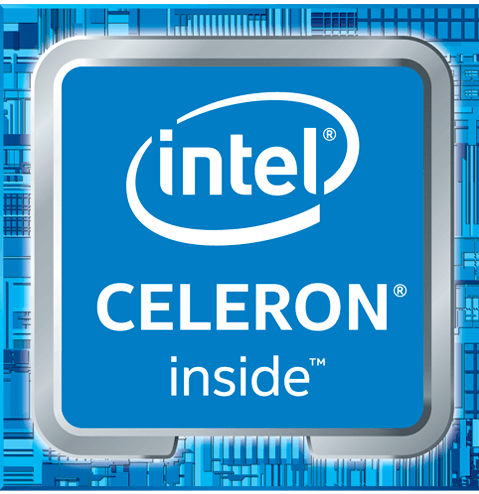
\includegraphics[width=1.75939in,height=1.80104in]{media/image18.png}
\end{figure}

% \hypertarget{pentium-iii-and-pentium-iii-xeon}{%
% \section{1999: Pentium III and Pentium III
% Xeon}\label{pentium-iii-and-pentium-iii-xeon}}

% The Pentium III was released in 1999 and was Intel's initial contender
% in the gigahertz race with AMD as well as the CPU that countered the
% low-power challenge from Transmeta in early 2000. The chip was initially
% released with the 250 nm Katmai core and was quickly scaled down to 180
% nm with Coppermine, Coppermine T and to 130 nm with the Tualatin core.

% The transistor count jumped from 9.5 million in Katmai to 28.1 million
% in the following cores due to the integrated L2 cache. The initial clock
% speed was 450 MHz and eventually reached 1,400 MHz with Tualatin. Intel
% was criticized to have rushed out the first gigahertz versions to
% compete with AMD's Athlon, which forced the company to recall its
% gigahertz processors and re-release them at a later time.

% Also noteworthy on the consumer side was the announcement of the Mobile
% Pentium III in 2000, which introduced SpeedStep and a scaling ability of
% clock speed of the processor, depending on its operation mode. The
% Mobile Pentium III was announced one day before the announcement of the
% Transmeta Crusoe processor, and many still believe tthat the Mobile
% Pentium III would not have been released without the pressure of
% Transmeta, which was famous for employing Linux inventor Linus Torvalds.

% The Pentium III Xeon was the last Xeon processor tied to the Pentium
% brand. The chip was released with the Tanner core in 1999. On the
% controversy side, Intel introduced the PSN, a Processor Serial Number,
% with the Pentium III. The feature caused several privacy complaints, and
% Intel eventually removed the feature and did not carry it over to future
% CPUs.

% \begin{figure}[ht!]
% 	\centering
% 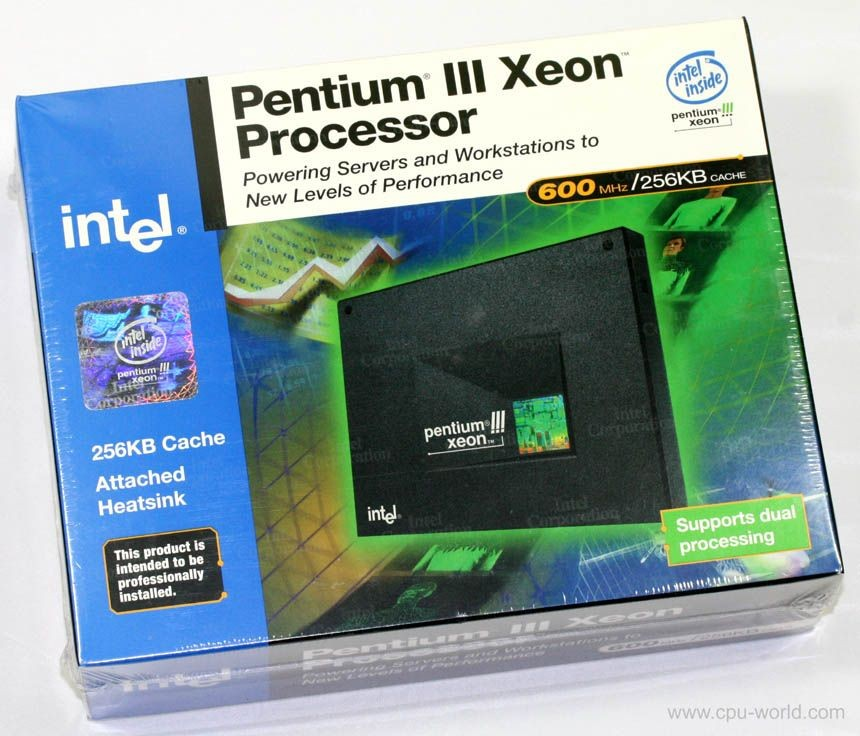
\includegraphics[width=3.57433in,height=3.06667in]{media/image19.jpeg}
% \end{figure}

\hypertarget{pentium-4}{%
\section{2000: Pentium 4}\label{pentium-4}}

The Pentium 4 arguably took Intel on a path that led to the most
dramatic transformation of Intel in the company's history. Launched in
2000 with the 180 nm Willamette core (42 million transistors), the
chip's Netburst architecture was designed to scale with clock speed, and
Intel envisioned that the foundation would allow the company to hit
frequencies of more than 20 GHz by 2010. Netburst, however, was more
limited than initially thought, and by 2003, Intel knew that the current
leakage and power consumption was increasing with higher clock speeds
too fast.

Netburst launched with 1.3 and 1.4 GHz, increased to 2.2 GHz with the
130 nm Northwood core (55 million transistors) in 2002, and to 3.8 GHz
with the 90 nm Prescott core (125 million transistors) in 2005. Intel
also launched the first Extreme Edition processors with the Gallatin
core in 2003.

Over time, the Pentium 4 series became increasingly confusing, with
Mobile Pentium 4-M processors, Pentium 4E HT (hyperthreading) processors
with support for a virtual

second core, and Pentium 4F processors with the 65 nm Cedar Mill core
(Pentium 4 600 series) in 2005. Intel planned to replace the Pentium 4
family with the Tejas processor, but canceled the project when it was
clear that Netburst would not be able to reach clock speeds beyond 3.8
GHz. Core, the following architecture, was a dramatic turnaround to much
more efficient CPUs with a strict power ceiling that put Intel's
gigahertz machine in reverse.

\begin{figure}[ht!]
	\centering
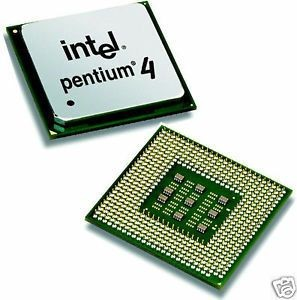
\includegraphics[scale=0.5]{media/image20.jpeg}
\end{figure}

\hypertarget{xeon}{%
\section{2001: Xeon}\label{xeon}}

The first Xeon that did not bring the Pentium brand along was based on
Pentium 4's Netburst architecture and debuted with the 180 nm Foster
core. It was available with 1.4 to 2.0 GHz clock speeds. The Netburst
architecture continued until 2006, when Intel had expanded Xeon to a
full line of UP and MP processors with the 90 nm Nocona, Irwindale,
Cranford, Potomac and Paxville cores and the 65 nm Dempsey and Tulsa
cores.

Similar to its desktop processors, the Netburst processors suffered from
excessive power consumption, which forced Intel to revise its processor
architecture and strategy. The Netburst Xeons died with the dual-core
Dempsey CPU with a clock speed of up to

3.73 GHz and 376 million transistors.

Today's Xeons are still based on the technology foundation that is also
used for desktop and mobile processors, but Intel keeps them in a tight
power envelope. The 2006

dual-core Woodcrest chip, a variant of the desktop Conroe chip, was the
first

representative of this new idea. The current Xeons are based on 32 nm
Sandy Bridge and Sandy Bridge EP architecture, and Westmere processor
designs. The CPUs have up to 10 cores and clock speeds up to 3.46 GHz,
as well as up to 2.6 billion transistors.

\begin{figure}[ht!]
	\centering
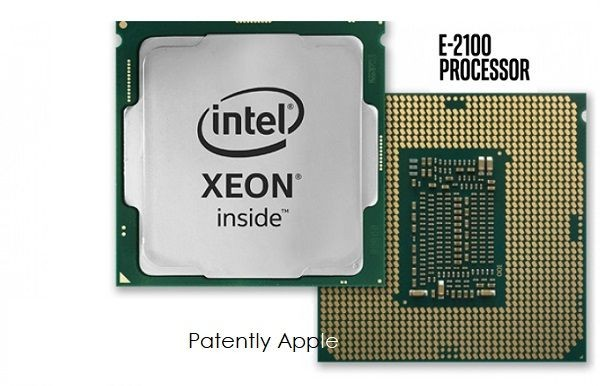
\includegraphics[scale=0.5]{media/image21.jpeg}
\end{figure}

\hypertarget{itanium}{%
\section{2001: Itanium}\label{itanium}}

The Itanium has been Intel's most misunderstood processor that actually
survived over a long period of time. While it follows the idea of the
i860 and iAPX 432, it has found some powerful supporters and not been
cut yet. The processor was launched as Intel's first

64-bit processor and was believed to be Intel's general idea for a
64-bit platform. However, the Itanium suffered in the 32-bit department
and was heavily criticized for its lack of performance in this segment.

Itanium was launched with the 180 nm Merced core in 2001 as a mainframe
processor with 733 MHz and 800 MHz clock speed and 320 million
transistors -- more than six times the count of a desktop Pentium at the
time. The Itanium 2 followed in 2002 (180 nm McKinley core, as well as
130 nm Madison, Deerfield, Hondo, Fanwood and Madison cores) and wasn't
updated until 2010 when Intel launched the Itanium 9000 with the 90 nm
Montecito and Montvale cores, as well as the 65 nm Tukwila core with a
massive 24 MB on-die cache, as well as more than 2 billion transistors.

Despite persistent rumors that Intel will kill the Itanium at any time,
there is a solid service ecosystem surrounding the processor.

\begin{figure}[ht!]
	\centering
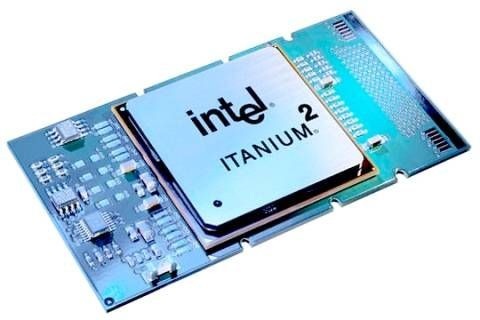
\includegraphics[scale=0.5]{media/image22.jpeg}
\end{figure}

\hypertarget{pentium-m}{%
\section{2003: Pentium M}\label{pentium-m}}

The Pentium M 700 series, launched with the 130 nm Banias core in 2003,
was targeted at mobile computers but carried the philosophy of an Intel
that did not focus its processors on clock speed anymore, but on power
efficiency. The processor was developed by Intel's design team in
Israel, which was led by Mooly Eden and David Perlmutter, who both hold
key executive roles at Intel today.

Banias dropped its clock speed to 900 MHz to 1.7 GHz, down from 2.6 GHz
of the Pentium 4 Mobile. However, the processor was rated at just 24.5
watts TDP, while the Pentium 4 chip was at 88 watts. The 90 nm shrink
was called Dothan and dropped its thermal design power to 21 watts.
Dothan had 140 million transistors and clock speeds of up to 2.13 GHz.

The direct successor of Dothan was Yonah, which was released in 2006 as
Core Duo and Core Solo, but was not related to the Intel Core
micro-architecture. The Banias core and its impact on Intel is seen on
the same level as the 4004, 8086 and 386 as the most significant
milestones in the company's product history.

\begin{figure}[ht!]
	\centering
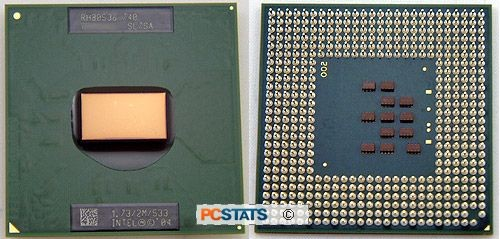
\includegraphics[scale=0.5]{media/image23.jpeg}
\end{figure}

:% \hypertarget{pentium-d}{%
% \section{2005: Pentium D}\label{pentium-d}}

% The Pentium D was Intel's first dual-core processor. Still based on
% Netburst, the first version had the 90 nm Smithfield core (two Northwood
% cores) and was released as the Pentium D 800 series. It was succeeded by
% the 65 nm Presler (with two Cedar Mill cores) dual-core.

% Intel also released Extreme Editions of both processors and capped the
% maximum clock speed at 3.73 MHz and at a power consumption of 130 watts
% -- the highest ever for any Intel consumer desktop processor (some
% server processors went up to 170 watts).

% Smithfield had 230 million transistors, Prescott 376 million.

% \begin{figure}[ht!]
% 	\centering
% 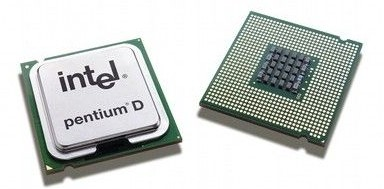
\includegraphics[width=3.793in,height=1.85062in]{media/image24.jpeg}
% \end{figure}

\hypertarget{core-2-duo}{%
\section{2006: Core 2 Duo}\label{core-2-duo}}

Core 2 Duo was Intel's strike back against AMD's Athlon X2 and Opteron
processors, which were highly successful at the time. The Core
micro-architecture was launched with the 65 nm Conroe (Core 2 Duo E-6000
series) on the desktop, Merom on the mobile side (Core 2 Duo T7000
series), and Woodcrest in the server market (Xeon 5100 series). Intel
quickly followed with quad-core versions (Kentsfield Core 2 Quad series
for the desktop, Clovertown Xeon 5300 series for servers).

The Core micro-architecture was preceded by one of the most significant
restructurings at Intel, as well as a substantial repositioning of the
company. While Conroe was developed, Intel positioned its remaining
Pentium and Pentium D processors to drive AMD into an unprecedented
price war in 2005 and 2006, while the Core 2 Duo processor regained the
performance lead over AMD in 2006. Conroe was launched with 1.2 GHz to 3
GHz clock speeds and as a chip with 291 million transistors. The CPUs
were updated with a 45 nm Penryn shrink in 2008 (Yorkfield for
quad-cores).

\begin{figure}[ht!]
	\centering
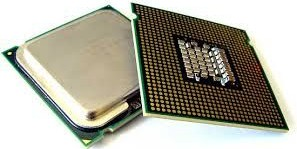
\includegraphics[scale=0.5]{media/image25.jpeg}
	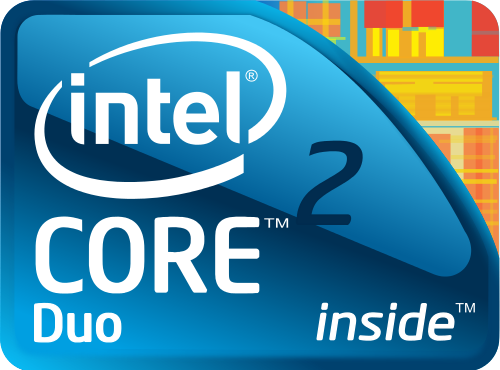
\includegraphics[scale=0.2]{media/image26.png}
\end{figure}

\section{2008: Core i-Series}

Intel's Core-i3, i5 and i7 processors launched with the Nehalem
micro-architecture and the company's 45 nm production process in 2008.
The architecture was scaled to 32 nm (Westmere) in 2010 and provided the
foundation for Intel processors covering the Celeron, Pentium Core and
Xeon brands. Westmere scaled to up to eight cores, up to

3.33 GHz clock speed and up to 2.3 billion transistors.

Westmere was effectively replaced by the 32 nm Sandy Bridge architecture
in 2011, which shrunk in 2012 to 22 nm in the Ivy Bridge generation (1.4
billion transistors for quad-core processors).

\begin{figure}[ht!]
	\centering
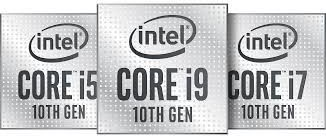
\includegraphics[scale=0.5]{media/image27.jpeg}
\end{figure}

\subsection{Intel Core First Generation - Nehalem}

\begin{itemize}
	\item The first Core i7 released by Intel was given the codename “Bloomfield”.
	\item Released in Q4 of 2008.
	\item 45 nm technology size
	\item Quad-Core Design with a shared L3 cache between the four different cores.
	\item Each core has a split  8-way set  associat ive L1 cache and a unified 8-way set  associat ive L2 cache.
	\item To further improve the effectiveness of the cache, Intel added prefetching.
	\item Main memory controller reduced time taken to access main memory.
\end{itemize}

\subsection{Intel  Core i7 -Sandy Bridge}

\begin{itemize}
	\item First released in early 2011
	\item32 nm technology size
	\item Similar cache to the Bloomfield generation of i7.
	\item Integrated Graphics Processor on same die as cores.
	\item Improved integrated memory controller
\end{itemize}


\subsection{Intel Core i7 - Ivy Bridge}

\begin{itemize}
	\item 22 nm technology size
	\item Estimated 4\%-6\% gain in IPC
	\item Improvement in cache prefetching
	\item Virtualization of move operations
\end{itemize}

\subsection{Intel Core i7 - Haswell}

\begin{itemize}
	\item 22 nm Technology Size
	\item Increase in Reservation Stations from 6 to 8
	\item Additional integer ALUs and branch unit
	\item One of the highest rates of per-clock throughput at the time
\end{itemize}


\subsection{Intel Core i7 - Broadwell}

\begin{itemize}
	\item 14 nm technology size
	\item Released in Early 2015
	\item Estimated 5\% increase in IPC
	\item Increase in L3 cache size
	\item Not very successful, replaced within a few months
\end{itemize}

\subsection{Intel Core i7 - Sky lake}

\begin{itemize}
	\item 14 nm Technology size
	\item Released late 2015, a few months after Broadwell
	\item 10\% faster than Broadwell
\end{itemize}



% \nocite{*}
% % %Bibliogra*phy
%  \addcontentsline{toc}{section}{Bibliography}
%  \bibliographystyle{apalike}
%  \bibliography{bibliography}

\end{document}
